\section{Práctica 5}

\subsection{}

El grafo con mayor cantidad de nodos es el que menos aristas por nodo tenga, para una cantidad de aristas fija.

Si quiero que tengan al menos grado 3, planteo que $m = \frac{\sum_{i = 1}^{n}d(v_i)}{2}$, con $n$ la cantidad de nodos y $m$ de aristas.

Tengo 19 aristas, por lo que $19 = \frac{\sum_{i = 1}^{n}d(v_i)}{2} = \frac{\sum_{i = 1}^{n}3}{2} = \frac{3}{2}n$

Entonces $n = \lfloor \frac{19 \times 2}{3}\rfloor = 12$

El truncamiento es por los grados que no tienen el grado mínimo, ya que el numero de aristas que tengo puede no ser divisible por este grado, como ocurre en este caso.

\setcounter{subsection}{3}
\subsection{}

Supongo que no se cumple. Entonces existe algun grafo con $n > 2$ nodos en donde no existen 2 nodos con la misma cantidad de aristas, que es lo mismo que, todos los grados de sus nodos son distintos.

Si cada nodo tiene grado distinto, los grados de los nodos deben ser concecutivos, ya que pertenecen al intervalo $[0, n - 1]$, que tiene $n$ grados posibles, uno para cada nodo. Pero si tomo el subgrafo que forman todos los nodos excepto el nodo de grado 0, tengo un grafo en donde uno de sus nodos tiene grado igual a la cantidad de aristas ($n - 1$). Absurdo. Por lo tanto en todo grafo con $n > 2$ nodos, existe al menos un par de nodos con igual grado.

\setcounter{subsection}{5}
\subsection{}

$\Longrightarrow$ )

Se que el grafo es conexo, es decir, que para cualquier par de nodos que tome, hay un camino que los une. Entonces, si tomo cualquier partición de $V$ en dos subconjuntos disjuntos $V_1$ y $V_2$, con $v, w \in V_1$, $v', w' \in V_2$, existe un camino entre $v$ y $v'$ que pasa por $w$ y $w'$ siendo $e$ el eje de $G$ que une $V_1$ y $V_2$, con $e = (w, w')$. \\

$\Longleftarrow$ )

\subsection{}

El grafo de $n$ nodos no conexo con mayor cantidad de aristas $m$ que puede formarse es aquel que tiene un nodo aislado, y el resto de los nodos formando un subgrafo completo de $n - 1$ vértices. 

El grado de estos $n - 1$ nodos es de $n - 2$ cada uno. Por lo tanto, 

\begin{center}
$\sum_{i = 1}^{n - 1}d(v_i) = (n - 1)(n - 2) = 2m$
\end{center}

Entonces $m = \frac{(n - 1)(n - 2)}{2}$. Si tuviera una arista más, el grafo sería conexo ya que no existe otro vértice sin arista que no sea el vértice aislado. Por lo tanto, un grafo con más de $\frac{(n - 1)(n - 2)}{2}$ es conexo.

\setcounter{subsection}{8}
\subsection{}

Tomo un par de caminos simples de longitud máxima de un grafo $G$ conexo y supongo que no se cruzan, es decir que no tienen ningún vértice en común. Como el grafo es conexo, existe al menos un camino que va de $v$ a $w$, con $v, w \in G$ que conecta los caminos $c_1$ y $c_2$. Entonces es posible formar un camino de mayor longitud tomando los subcaminos máximos de cada camino de mayor longitud hasta $v$ y $w$, respectivamente, y el camino que los une, ya que los subcaminos máximos pasan por al menos la mitad de la longitud máxima de vértices y a eso le sumo un camino con al menos una arista. Absurdo. Por lo tanto,  todo par de caminos de longitud máxima comparten al menos un vértice.

\subsection{}

\subsubsection{}

Si un digrafo es fuertemente conexo quiere decir que existe un camino dirigido para cualquier par de vértices. Si tomamos su grafo subyacente, es decir, quitar la dirección en las aristas, seguiremos teniendo un camino para cualquier par de vértices. Por lo tanto, el grafo subyacente es conexo.

La implicación no funciona para el otro lado ya que si tenemos un grafo subyacente conexo, no es posible saber en qué dirección están las aristas de su grafo dirigido, por lo que no sabemos si es o no un grafo fuertemente conexo.

\subsubsection{}

$\Longrightarrow$ )

Sea $G$ un grafo conexo y orientable de forma que se convierta en un grafo fuertemente conexo, existe un camino de cada nodo a sí mismo, ya que al ser orientable a un grafo fuertemente conexo, existe un camino orientado para cualquier par de nodos. 

Tomo $u$ y $v$ dos nodos pertenecientes a $G$. Existe un camino orientado de $u$ a $v$, y también de $v$ a $u$. Al ser $G$ conexo y orientable, existe un único arco entre cada par de nodos. Entonces el camino que une $u$ con $v$, es distinto al que une $v$ con $u$, ya que no comparten arcos. Entonces $u$ y $v$ pertenecen a un circuito simple. \\

$\Longleftarrow$ )

Sea $G$ un grafo conexo donde cada eje pertenece a un circuito simple, sea el eje $E \in G$ con extremos $u$ y $v$, 

\subsubsection{}
Que todas las cuadras pertenezcan a un circuito simple.

\setcounter{subsection}{11}
\subsection{}

Una secuencia de números enteros no negativos $d_1,...,d_n$ es la secuencia de grados de un grafo

$\Longleftrightarrow \frac{\sum_{i = 1}^{n}d_i}{2} = m$ con $m$ la cantidad de aristas

$\Longleftrightarrow \sum_{i = 1}^{n}d_i = 2m$ es decir, $\sum_{i = 1}^{n}d_i$ es par

\subsection{}

\subsubsection{}
\begin{itemize}
\item (7,6,5,4,3,3,2) no puede ser secuencia gráfica ya que ningún nodo puede tener grado mayor o igual a la cantidad de nodos, y el primer elemento lo tiene.

\item (6,6,5,4,3,3,1) no puede ser secuencia gráfica ya que los primeros dos elementos estan unidos a todo el resto, y el último tiene grado 1, lo cual no es posible ya que es seguro que esta unido a los dos primeros elementos.
\end{itemize}

\subsubsection{}
Por $5.12$ sabemos que vale que $\sum_{i = 1}^{n}d_i$ es par.

$\sum_{i = k + 1}^{n}min(k, d_i)$

\subsection{}
Si $G$ tiene $n - 1$ vértices de grado impar, entonces $n - 1$ es par, por lo tanto $n$ es impar y hay un único nodo de grado par. Como $n$ es par, para $\overline{G}$ se invierte la cantidad de aristas quedando pares los grados impares, y viceversa.

\setcounter{subsection}{20}
\subsection{}
\subsubsection{}

\begin{center}
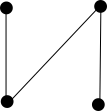
\includegraphics{imagenes/grafo_autocomplementario.png}
\end{center}

\subsubsection{}

Sabemos que $\sum_{i = 1}^{n}d(v_i) = 2m$ con $m$ la cantidad de aristas.

y que $\sum_{i = 1}^{n}d(\overline{v_i}) = \sum_{i = 1}^{n}n - 1 - d(v_i) = \sum_{i = 1}^{n}n - \sum_{i = 1}^{n}1 - \sum_{i = 1}^{n}d(v_i)$ 

Entonces $2\sum_{i = 1}^{n}d(v_i) = n^2 - n \Longleftrightarrow \sum_{i = 1}^{n}d(v_i) = \frac{n^2 - n}{2} = 2m$

Nos queda que $m = \frac{n(n - 1)}{4}$

El producto $n(n - 1)$ debe ser divisible por 4, y como no es posible que ambos sean pares, significa que uno de los factores debe ser divisible por 4. Lo que es lo mismo que $n = 4k$ ó $(n - 1) = 4k \Longleftrightarrow n = 4k + 1$

\subsection{}

\begin{codesnippet}
\begin{verbatim}
bool isomorfos?(arreglo<lista<int> U, arreglo<lista<int> V)

fin isomorfos?
\end{verbatim}
\end{codesnippet}

\subsection{}

Se copian todos los 1 en sus posiciones simetricas, es decir si $M_{ij} = M_{ji}$

\subsection{}

\subsubsection{}
$A^n$ contiene en cada elemento $A_{ij}$ la cantidad de caminos que hay de longitud $n$ desde $i$ hasta $j$.

\subsubsection{}
Sabemos que un grafo $G$ con 2 o más nodos es bipartito $\Longleftrightarrow$ no tiene circuitos simples de longitud impar.

Y también que si $A$ es la matriz de adyacencia del grafo $G$, el elemento $a^k$ de $A^k_{ij}$
es igual a la cantidad de caminos de longitud $k$ entre $i$ y $j$.

Entonces los elementos de la diagonal de $A^n$ representan la cantidad de circuitos simples de longitud $n$ para cada $A^n_{ii}$. Por lo que una diagonal nula representa que no hay circuitos simples de longitud $n$.

Por lo tanto vale que un grafo es bipartito $\Longleftrightarrow$ no tiene circuitos simples de longitud impar $\Longleftrightarrow$ la diagonal de $A^n$ con $n$ impar, es nula.

\subsection{}
Fijándose para cada $i, j$ con $1 \leq i, j \leq n$ si es posible llegar desde $i$ a $j$, si lo es se pone un 1, sino un 0. ESTO ES MALISIMO

\subsection{}
\subsubsection{}
BFS para detectar ciclos de longitud impar. La idea es que al tener el nivel de cada nodo, si se forma un ciclo y el nivel del nodo desde el que se mueve coincide en paridad con el del nodo al que llega, entonces hay un ciclo de longitud impar y no es bipartito. Si no se encuentra ninguno, es bipartito.

\begin{codesnippet}
\begin{verbatim}
bool bipartitoBFS(vector<vector<int> listaAdyacencia)

    cola<int> recorrido
    vector[n]<int> nivel
    vector[n]<bool> visitado

    // Mientras queden vertices sin visitar
    para i entre 0 y n
        si !visitado[i] entonces

            visitado[i] = verdadero
            nivel[i] = 0

            recorrido.encolar(i)
            mientras !recorrido.vacia?() hacer

                int actual = recorrido.desencolar()

                para j entre 0 y listaAdyacencia.tamaño()

                    int sucesor = listaAdyacencia[actual][j]

                    si visitado[sucesor] entonces
                        si nivel[actual] + nivel[sucesor] mod 2 == 0 entonces
                            devolver falso
                        fin si
                    sino

                        visitado[sucesor] = verdadero
                        nivel[sucesor] = nivel[actual] + 1
                        recorrido.encolar(sucesor)

                    fin si

                fin para
            fin mientras
        fin si
    fin para

    devolver verdadero

fin bipartitoBFS
\end{verbatim}
\end{codesnippet}

También se puede calcular todas las potencias impares de las matriz de adyacencia hasta $A^n$ y fijarse en la diagonal de cada una. Si se encuentra todas son nulas, es bipartito. Sino no lo es.

\subsubsection{}
Recorrer toda la matriz de adyacencia intercambiando 0s por 1s y viceversa

\subsubsection{}

\begin{itemize}
\item $\ord(n + m)$
\item $\ord(n^2)$
\end{itemize}

\subsection{}

\subsubsection{}
Cuento la cantidad de vecinos de cada vértice. Si alguno tiene un único vecino, entonces devuelvo falso. Si todos tiene 0 ó dos o mas vecinos, es verdadero.

\subsubsection{}
Primero se usa el algoritmo anterior para verificar si cada eje pertenece a un ciclo. Si es asi entonces es orientable de forma que quede fuertemente conexo, de lo contrario no lo es.

El resto del algoritmo es un DFS en el cual se da dirección a las aristas en el momento de moverse de nodo.

Elegir un nodo cualquiera.

Para ese nodo se elige un vecino y se marca su arista en direccion al mismo. Ahora se hace lo mismo para el vecino y así, recursivamente.

En algún momento se llega a un nodo ya visitado. Se vuelve en la pila de la recursión hasta encontrar un nodo al que le queden vecinos sin visitar y se vuelve a hacer el llamado recursivo para ese vecino.

\subsubsection{}
En ambos métodos lo conveniente es recibir el grafo como una lista de adyacencias.

\begin{itemize}
\item $\ord(n)$ ya que se fija en la cantidad de vecinos de cada nodo.
\item $\ord(n + m)$ ya que usa el algoritmo anterior y recorre todas las aristas, dos veces (una de ida y una de vuelta)
\end{itemize}

\subsection{}

\setcounter{subsubsection}{1}
\subsubsection{}

\begin{codesnippet}
\begin{verbatim}
maximales(vector<vector<int>> listaAdyacencia)

    vector<vector<int>> subgrafos

    mientras haya nodos sin visitar

        actual = nodoSinVisitar()
        para vecino <- actual.vecinos()

            lista<int> susVecinos = vecino.vecinos()

            // Si cada uno de sus vecinos tiene como vecino al resto y ninguno de sus vecinos 
            // marcados es vecino de actual, es un subgrafo completo maximal
            si vecinosEntreTodos?(susVecinos) && !vecinoMarcado(actual, susVecinos) entonces
                subgrafos.agregar(susVecinos + vecino + actual)
            fin si

            // Si tiene algun vecino que no sea vecino de actual, no se marca
            si todosVecinosDe(actual, susVecinos) entonces
                marcar(vecino)
            fin si

        fin para
    fin mientras

    devolver subgrafos

fin maximales
\end{verbatim}
\end{codesnippet}

\subsubsection{}
La complejidad de b. es monstruosa :)